%\documentclass[twocolumn]{emulateapj}
%\documentclass[12pt,preprint]{aastex}

\documentclass[usenatbib]{mn2e}

\newcommand{\s}{$_{\rm s}$}
\newcommand{\kms}{km~s$^{-1}$}
\newcommand{\msun}{{\it M}$_{\odot}$}
\newcommand{\lsun}{{\it L}$_{\odot}$}
\newcommand{\mear}{{\it M}$_{\oplus}$}
\newcommand{\etal}{{\it et al.}}
\newcommand{\ie}{{\it i.e.}}
\newcommand{\eg}{{\it e.g.}}
\newcommand{\be}{\begin{equation}}
\newcommand{\ee}{\end{equation}}
\newcommand{\magarc}{{\rm mag\,arcsec$^{-2}$}}
\newcommand{\MK}{{{\rm M}_{\rm ext,K}-5\log h}}
\newcommand{\ri}{{$r_{21}$}}
\newcommand{\ra}{$R_A$}
\newcommand{\vobs}{{v_{\rm obs}}}
\newcommand{\kmsMpc}{km~s$^{-1}$ Mpc$^{-1}$}
\newcommand{\h}{$h_{70}$}
\newcommand{\vpec}{v_{\rm pec}}
\newcommand{\like}{{\mathcal L}}
\newcommand{\vs}{\vspace*{5pt}}
\newcommand{\continued}{ (Continued)}

% Journals
\newcommand{\mnras}{MNRAS}
\newcommand{\apj}{ApJ}
\newcommand{\apjl}{ApJL}
\newcommand{\aj}{AJ}
\newcommand{\pasp}{PASP}
\newcommand{\aaps}{A\&AS}
\newcommand{\aap}{A\&A}
\newcommand{\apjs}{ApJS}
\newcommand{\araa}{ARA\&A}
\newcommand{\pbar}{p_{\rm bar}}
\newcommand{\fHI}{f_{\rm HI}}

\voffset-1.25cm

\usepackage{epsfig}
\begin{document}

\title[Galaxy Zoo Hubble Data]{Galaxy Zoo: Classifications for Galaxies in HST Legacy Imaging}
%Bars Regulating Star Formation though the Atomic Gas Content of Disc Galaxies}
%The Atomic Gas Content of Barred Galaxies from ALFALFA$^*$: Bar Feedback in Intermediate Mass Disc Galaxies }
\author[Lead Author \etal]{Lead Author and other Galaxy Zoo science team\\
%$^1$Institute for Cosmology and Gravitation, University of Portsmouth, Dennis Sciama Building, Burnaby Road, Portsmouth, PO1 3FX, UK \\
%$^2$South East Physics Network, www.sepnet.ac.uk\\
%$^3$Dept. of Astronomy, Cornell University, Space Sciences Building, Ithaca, NY 14850, USA\\
 %$^2$Institute for Sciences of the Cosmos (ICCUB), University of Barcelona, Marti i Franques 1, Barcelona, 08024 Spain\\
% $^{4}$Oxford Astrophysics, Department of Physics, University of Oxford, Denys Wilkinson Building, Keble Road, Oxford, OX1 3RH, UK\\
%$^{5}$Yale Center for Astronomy and Astrophysics, Yale University, P.O. Box 208121, New Haven, CT 06520, USA \\
%$^6$Steward Observatory, University of Arizona, 933 N. Cherry Ave, Tuscon, AZ 85721, USA\\
 %$^4$Astronomy Department, Adler Planetarium and Astronomy Museum, 1300 Lake Shore Drive, Chicago, IL 60605, USA\\
 % $^7$Centre for Astronomy \& Particle Theory, University of Nottingham, University Park, Nottingham, NG7 2RD, UK\\
 %$^6$School of Physics and Astronomy, University of Minnesota, Minneapolis, MN 55455, USA\\
 %$^7$Department of Physics \& Astronomy, 206 Gallalee Hall, 514 University Blvd., University of Alabama, Tuscaloosa, AL 35487-0234, USA\\
% $^8$Einstein Fellow\\ 
\\
 $^*$This publication has been made possible by the participation of more than 200,000 volunteers in the Galaxy Zoo project. \\ Their contributions are individually acknowledged at \texttt{http://www.galaxyzoo.org/volunteers}. \\
\\
{\tt E-mail: lead.author@university.edu}
 }

%\date{Accepted for publication in MNRAS, 7th October 2010.}
%\pagerange{1--10} \pubyear{2010}

\maketitle

\begin{abstract}

Data release paper for GZ Hubble

\end{abstract}

%\keywords{galaxies: distances and redshifts --- galaxies: clusters --- galaxies: fundamental parameters --- distance scale --- cosmological parameters}

\section{Introduction}


\section{Sample and Data} 

\subsection{Summary of HST Legacy Survey Imaging}

\begin{itemize}
\item AEGIS has1 orbit each (~2200 seconds) in F606W (V band) and F814W filter and has been dithered to 0.03 ''/pixel; the imaging covers ~710 arcmin$^2$.

\item GOODS targeted 2 fields, GOODS-N and GOODS-S, imaging in 4 filters -- F435W (B), F606W (V), F775W (i), and F850LP (z). The mean exposure times vary, from 1000 - 2100 seconds. The images have been dithered to a pixel scale of 0.03 ''/pixel and covers at total area of ~320 arcmin$^2$ (160 arcmin$^2$ per field). The filters that Griffith et al uses for the colored images were F606W and F775W for GOODS-N and F606W and F850LP for GOODS-S.

\item COSMOS has 1 orbit (2028 seconds) in the F814W (I band) filter and has been dithered to 0.05 ''/pixel; it covers the largest area, ~1.8 deg$^2$. 

\item GEMS has 1 orbit (2160 and 2286 seconds) in the F606W and F850LP filters, with a pixel scale of 0.03 ''/pixel; it covers ~800 arcmin$^2$
\end{itemize}

\section{Correcting for Redshift Dependent Classification Bias}

We can't do what we did in Bamford et al. (2009) for the original GZ or Willett et al. (2013) for GZ2 because these both depended on the assumption of no redshift bias. In the GZH samples the redshift range is so large that we expect to find redshift evolution of the types and morphologies of galaxies which are seen. 

We also expect to see changes in the apparent morphology of galaxies due to band shifting and surface brightness effects (e.g. see Figure \ref{redshift} which illustrates one possible effect of losing features in spiral galaxies at high redshift). So we need to measure this. 

\begin{figure}
\includegraphics[width=60mm]{example_ferengi2.ps}
%\includegraphics[height=80mm,angle=-90]{TuningFork.ps}
\caption{Examples of an obvious spiral and obvious elliptical at $z=0$ which both look similar when redshifted to $z=0.8$. See below for the description of the method for redshirting.  \label{exampleFERENGI}}
\end{figure}
 


So we made images of the same galaxy at a variety of redshifts using input images from the SDSS (cite the SDSS) and the FERENGI code (cite Ferengi) to produce images from these typical of those observed in the HST surveys. 
 
\subsection{Selection of FERENGI Input Galaxies}






We select 288 different galaxies in SDSS imaging to run through the FERENGI code.

The selection spanned a variety of galaxy morphologies (as indicated by GZ2 classifications), with a range of surface brightnesses, and also picked ideal {\bf need Edmond to fill in} for different target redshifts in HST imaging. 

 The selection criteria for the different morphological categories is summarised in Table \ref{morphologies}. The surface brightness selection was (1) low: $\mu > 21.5 {\rm mag arsec}^2$;  (2) mid: $20.5 < \mu < 21.5 {\rm mag arsec}^2$; and (3) high: $\mu < 20.5 {\rm mag arsec}^2$. 
 
\begin{table*}
\caption{Summary of morphological categories \label{morphologies}}
\begin{tabular}{lllc}
\hline\hline
Morphology & Label &  Selection & $N_{\rm objects}$ \\
\hline
Features & Yes & $p_{\rm features} > 0.8$, $p_{rm odd} < 0.1$ & 12 \\ 
 & Int & $0.3 < p_{\rm smooth} < 0.6$, $p_{\rm odd} < 0.1$ & 12 \\ 
 & No &  $p_{\rm smooth} > 0.8$, $p_{\rm odd} < 0.1$ & 12 \\ 
Merger & No & $p_{\rm features} > 0.8$, $p_{\rm odd < 0.1}$, $p_{\rm merger} < 0.1$ & 12\\
& Int & $p_{\rm odd} > 0.5$, $0.1< p_{\rm merger} < 0.4$ & 12 \\ 
& Yes & $p_{\rm odd} > 0.5$, $p_{\rm merger} > 0.4$ & 12\\
Edge-on & Yes &  $p_{\rm edgeon} > 0.8$, $p_{\rm features} > 0.5$ & 12 \\
& Int & $0.4 < p_{\rm edgeon} < 0.8$ , $p_{\rm features} > 0.5$ & 12 \\
& No & $p_{\rm edgeon} < 0.2$, $p_{\rm features} > 0.5$ & 12 \\
Bar & No & $p_{\rm bar} < 0.1$, $p_{\rm features} > 0.5$, $p_{\rm edgeon} < 0.2$ & 24 \\
& Int & $0.2 < p_{\rm bar} < 0.4$, $p_{\rm features} > 0.5$, $p_{\rm edgeon} < 0.2$ & 24 \\
& Yes&  $p_{\rm bar} > 0.8$, $p_{\rm features} > 0.5$, $p_{\rm edgeon} < 0.2$ & 24 \\
Visible spiral & No & $p_{\rm spiral} < 0.2$, $p_{\rm features} > 0.5$, $p_{\rm edgeon} < 0.2$, $p_{\rm bar} < 0.1$ & 12 \\
& Int &  $0.2 < p_{\rm spiral} < 0.8$, $p_{\rm features} > 0.5$, $p_{\rm edgeon} < 0.2$, $p_{\rm bar} < 0.1$ & 12 \\
& Yes &  $p_{\rm spiral} > 0.8$, $p_{\rm features} > 0.5$, $p_{\rm edgeon} < 0.2$, $p_{\rm bar} < 0.1$ & 12 \\
Oblique Bulge Size & No & $p_{\rm nobulge>0.6}$, $p_{\rm features} > 0.5$, $p_{\rm edgeon} < 0.5$, $p_{\rm bar} < 0.2$ & 12 \\
& Int &  $p_{\rm justnoticeable}>0.6$, $p_{\rm features} > 0.5$, $p_{\rm edgeon} < 0.5$, $p_{\rm bar} < 0.2$ & 12 \\
& Yes & $p_{\rm obvious/dominent}>0.5$\footnote{Edmond does this means $p_{\rm obv}+p_{\rm dom}>0.5$ or $p_{\rm ob} OR p_{\rm dom} >0.5$? }, $p_{\rm features} > 0.5$, $p_{\rm edgeon} < 0.5$, $p_{\rm bar} < 0.2$ & 12 \\
Edge-on bulge shape 
& Round & $p_{\rm rounded}>0.5$, $p_{\rm features} > 0.5$, $p_{\rm edgeon} > 0.5$ & 12\\
& Boxy & $p_{\rm boxy}>0.4$, $p_{\rm features} > 0.5$, $p_{\rm edgeon} > 0.2$ & 12\\
& Non & $p_{\rm nobulge}>0.5$, $p_{\rm features} > 0.5$, $p_{\rm edgeon} > 0.5$ & 12\\
\hline\hline
\end{tabular}
\end{table*}

There were four ``target redshifts" ($z = 0.3, 0.5, 0.8$ and 1.0), and from these points the images were redshifted in $\Delta z = 0.1$ bins up to $z=1.0$. In addition different evolution models were assumed in FERENGI. This evolution is a crude mechanism that is suppose to mimic the brightness increase of galaxies with increasing redshift. The evolution mechanism allows us to make galaxies brighter as linear function of redshift, and that is it. It is an empirical addition to the magnitude of a galaxy of the form $M' = e z + M$, where $M'$ is the corrected magnitude, $e$ is the evolutionary correction in magnitudes.  (i.e. $e=-1$ essentially brightens the galaxy by 1 magnitude by $z=1$). {\bf What values of $e$ did we use?} Depending on the target, or starting redshift we ran FERENGI for several final redshifts and different evolution models as summarized in Table \ref{ferengi}. 

\begin{table}
\caption{Summary of FERENGI runs \label{ferengi}}
\begin{tabular}{lccccc}
\hline\hline
Starting redshift &  $N_{z {\rm bins}}$ & $N_{\rm evolution}$ & $N_{\rm runs}$ & $N_{\rm total}$\\
\hline
0.3 & 8 & 7 & 56 & 4031 \\
0.5 & 6 & 4 & 24 & 1728 \\
0.8 & 3 & 3 & 9 & 648 \\
1.0 & 1 & 3 & 3 & 216 \\
\hline\hline
\end{tabular}
\end{table}

Two series of example redshifted images are shown in Figure \ref{exampleFERENGI}.

\begin{figure*}
\includegraphics[width=160mm]{example_ferengi.ps}
%\includegraphics[height=80mm,angle=-90]{TuningFork.ps}
\caption{Examples of two galaxies which have been run through the FERENGI code to produce simulated HST images. \label{exampleFERENGI}}
\end{figure*}
 

\subsection{Results of FERENGI Analysis}

We show here the {\bf currently fake} results of citizen scientist classifications of images of galaxies placed at artificial redshifts. Figure \ref{results1} shows the {\bf currently fake} change of vote fractions for feature X with redshift, for three vote fraction levels with three surface-brightness levels and 7 evolutionary corrections. 

%-----------------------------------------------------------------------------------------------------------------------------------
\begin{figure}
\begin{center}

\includegraphics[width=0.35\textwidth,angle=90]{fake_results.ps}

\caption{Fake results of the FERENGI redshifting exercise. For three vote fraction levels with three surface-brightness levels and 7 evolutionary corrections each, we show the evolution of the vote fractions for feature X with redshift.}

\label{fig:ferengi_results_fake}

\end{center}
\end{figure}
%-----------------------------------------------------------------------------------------------------------------------------------




\section{Summary}

 
\paragraph*{ACKNOWLEDGEMENTS.} 

This publication has been made possible by the participation of more than 200,000 volunteers in the Galaxy Zoo project. Their contributions are individually acknowledged at \texttt{http://www.galaxyzoo.org/volunteers}. Galaxy Zoo 2 was developed with the help of a grant from The Leverhulme Trust. KS gratefully acknowledges support from Swiss National Science Foundation Grant PP00P2\_138979/1.

HST acknowledgements.

Funding for the SDSS and SDSS-II has been provided by the Alfred P. Sloan Foundation, the Participating Institutions, the National Science Foundation, the U.S. Department of Energy, the National Aeronautics and Space Administration, the Japanese Monbukagakusho, the Max Planck Society, and the Higher Education Funding Council for England. The SDSS Web Site is http://www.sdss.org/. 

The SDSS is managed by the Astrophysical Research Consortium for the Participating Institutions. The Participating Institutions are the American Museum of Natural History, Astrophysical  Institute Potsdam, University of Basel, University of Cambridge, 
Case Western Reserve University, University of Chicago, Drexel University, Fermilab, the Institute for Advanced Study, the Japan 
Participation Group, Johns Hopkins University, the Joint Institute for Nuclear Astrophysics, the Kavli Institute for Particle Astrophysics and Cosmology, the Korean Scientist Group, the Chinese Academy of Sciences (LAMOST), Los Alamos National Laboratory, the Max-Planck-Institute for Astronomy (MPIA), the Max-Planck-Institute for Astrophysics (MPA), New Mexico State Uni- 
versity, Ohio State University, University of Pittsburgh, University of Portsmouth, Princeton University, the United States Naval Observatory and the University of Washington. 


\begin{thebibliography}{}

\end{thebibliography}

\end{document}
